\documentclass[a4paper, 12pt, oneside]{book}

%\usepackage[T1]{fontenc}
\usepackage[utf8]{inputenc}

\usepackage[english]{babel}
\usepackage{geometry}
\usepackage{hhline}
\usepackage{amsthm}
\usepackage{amsmath}
\usepackage{amssymb}
\usepackage{comment}
\usepackage{enumerate}
\usepackage{mathrsfs}
\usepackage{multirow}
\usepackage{fullpage}
\usepackage{indentfirst}
\usepackage{color}
\usepackage{courier}
\usepackage{afterpage}
\usepackage{url}
\usepackage{float}
\usepackage{tabularx}
\usepackage[hidelinks]{hyperref}
\usepackage{cleveref}
\usepackage{epsfig}
\usepackage{pdfpages}
\usepackage{lastpage}
\usepackage{caption}
\usepackage{subcaption}
\usepackage{tikz}
\usepackage{siunitx}
\usepackage{listings}
\usepackage{lipsum}

\usepackage{setspace}
\usepackage{fancyhdr}

\renewcommand{\chaptermark}[1]{%
\markboth{\MakeUppercase{%
\chaptername}\ \thechapter.%
\ #1}{}}
\pagestyle{fancy}
\fancyhf{}
\fancyhead[L]{\leftmark}
\fancyhead[R]{\thepage}

\setlength{\headheight}{15pt}
\setlength{\headsep}{20pt}

\fancypagestyle{plain}{
  \fancyhf{} 
  \renewcommand{\headrulewidth}{0pt}
  \renewcommand{\footrulewidth}{0pt}
  \renewcommand{\headheight}{0pt}
  \renewcommand{\headsep}{0pt}
}

\usetikzlibrary{matrix,decorations.pathmorphing}

\graphicspath{/Users/alexandergodal/Desktop/BP/latex/img} 

\hypersetup{
    colorlinks=false,
    linkcolor=red,
    filecolor=magenta,      
    urlcolor=cyan,
    citecolor=blue
}

\usepackage{booktabs}

%%%%%%%%%%%%%%%%%%%%%%%%%%%%%%%%%%%%%%%%%
%%%% General macros %%%%%%%%%%%%%%%%%%%%%
%%%%%%%%%%%%%%%%%%%%%%%%%%%%%%%%%%%%%%%%%

\newcommand{\cvuten}{Czech Technical University in~Prague}
\newcommand{\fjfien}{Faculty of Nuclear Sciences and Physical Engineering}
\newcommand{\kfen}{Department of Physics}
\newcommand{\oboren}{Nuclear and Particle Physics}

\newcommand{\cvut}{České vysoké učení technické v Praze}
\newcommand{\fjfi}{Fakulta jaderná a fyzikálně inženýrská}
\newcommand{\kf}{Katedra fyziky}
\newcommand{\obor}{Jaderná a částicová fyzika}

\newcommand{\nazevcz}{Simulace hadronového kalorimetru nHCal pro ePIC experiment}
\newcommand{\klicovaslovacz}{EIC, experiment ePIC, hadronový kalorimetr}
\newcommand{\abstraktcz}{}

\newcommand{\nazeven}{Simulation of hadronic calorimeter nHCal for ePIC experiment} %skontrolovať názov – Hadron(-ic)
\newcommand{\klicovaslovaen}{EIC, ePIC Experiment, Hadronic Calorimeter}
\newcommand{\abstrakten}{}



\newcommand{\autor}{Bc. Alexander Godál}           
\newcommand{\rok}{2025}                 
\newcommand{\vedouci}{doc.~Mgr.~Jaroslav~Bielčík,~Ph.D.}
\newcommand{\konzultant}{Ing.~Alexandr~Prozorov,~Ph.D.}  

\newcommand{\akrok}{2024/2025}

\newcommand{\prohlaseni}{}

                                                               
%%%%%%%%%%%%%%%%%%%%%%%%%%%%%%%%%%%%%%%%
%%%%% Setting %%%%%%%%%%%%%%%%%%%%%%%%%%
%%%%%%%%%%%%%%%%%%%%%%%%%%%%%%%%%%%%%%%%

%\oddsidemargin=10mm  
%\topmargin=-15mm     
\textwidth=150mm     
\textheight=240mm     


\pagenumbering{arabic}  

%\parindent=0pt 
%\parskip=7pt   
\frenchspacing
%\linespread
\setlength{\abovecaptionskip}{8pt plus 3pt minus 3pt}

%%%%%%%%%%%%%%%%%%   Particles Macros  %%%%%%%%%%%%%%%%%%%%%%%%%%%%%

\newcommand{\my}[1]{{\rm #1}}

\newcommand{\proton}{\my{p}}

\newcommand{\higgs}{\my{H}}
\newcommand{\gluon}{\my{g}}
\newcommand{\pik}{\ensuremath{\pi/\my{K}}}

\newcommand{\photon}{\gamma}
\newcommand{\wboson}{W}
\newcommand{\zboson}{Z}

\newcommand{\electron}{e^-}
\newcommand{\muon}{\mu^-}
\newcommand{\tauon}{\tau^-}

\newcommand{\eneutrino}{\nu_e}
\newcommand{\mneutrino}{\nu_\mu}
\newcommand{\tneutrino}{\nu_\tau}

\newcommand{\qu}{u}
\newcommand{\qd}{d}
\newcommand{\qc}{c}
\newcommand{\qs}{s}
\newcommand{\qt}{t}
\newcommand{\qb}{b}

%%%%%%%%%%%%%%%%%%%%%%%%%%%%%%%%%%%%%%%%%%%%%% Personal Macros %%%%%%%%%%%%%%%%%%%
%%%%%%%%%%%%%%%%%%%%%%%%%%%%%%%%%%%%%%%%% 

%\newcommand{\oo}{\texttt{O$^2$}}
\newcommand{\ROOT}{ROOT}

\newcommand{\e}{\mathrm{e}}
\newcommand{\Lowq}{Low\,-\,\ensuremath{Q^2}~}
\newcommand{\lowq}{low\,-\,\ensuremath{Q^2}~}

\newcommand{\cor}[1]{\textcolor[rgb]{1,0,0}{#1}}
%\def\cor{}
\newcommand{\keep}[1]{\textcolor[rgb]{0,1,0}{#1}}

\newcommand{\clarify}[1]{\textcolor[rgb]{0,0,1}{#1}}

\newcommand{\abs}[1]{\lvert #1 \rvert}
\newcommand{\diff}[1]{\text{d}#1}

\newcommand{\R}{\mathbb{R}}
\newcommand{\sv}[2]{\forall^{\star} #1 \in #2}

\newcommand{\maybegeq}{\overset{?}{\geq}}

\newcommand{\dol}[1]{_{\text{#1}}}
\newcommand{\hor}[1]{^{\text{#1}}}
\newcommand{\bra}[1]{\ensuremath{\langle #1 |}}
\newcommand{\ket}[1]{\ensuremath{| #1 \rangle}}
\newcommand{\braket}[2]{\ensuremath{\left\langle #1 | #2 \right\rangle}}
%\let\theta\vartheta


%%%%%%%%%%%%%%%%%%%%%%%%%%%%%%%%%%%%%%%%%%%%% Document %%%%%%%%%%%%%%%%%%%%%%%%%%%%%%%%%%%%%%%%%%%%%%%%%%%%%%%%%%%%%%%%%%%%
\begin{document}

%%%% 1. strana (Titulni strana) %%%%%%%%

\thispagestyle{empty}

\begin{center}

{\large \bf \cvut} 
    
{\large \bf \fjfi}
    
\vspace{15mm}

{\large \bf \kf} 
    
{\large \bf \obor}
    
\vspace{10mm} 

\epsfysize=30mm 
\epsffile{img/logo_FJFI.pdf}  

\vspace{15mm}
  
{\Large VÝZKUMNÝ ÚKOL}

\vspace{15mm}
   
   
{\Huge \bf \nazevcz} 
 

\vspace{6mm}

   
   \vfill
   {\large
    
    Praha, 2025 \hfill \autor}
\end{center}

%%%%%%%%%%%%%%%%%%%%%%%%%%%%%%%%%%%%%%%%%%%%%%%%%%%%%%%%%%%%%%%%%%%%%%%%%%%%%%%
\newpage
%%%%%%%%%%%%%%%%%%%%%%%%%%%%%%%%%%%%%%%%%%%%%%%%%%%%%%%%%%%%%%%%%%%%%%%%%%%%%%%

\thispagestyle{empty}

\begin{center}

{\large \bf \cvuten} 
    
{\large \bf \fjfien}
    
\vspace{15mm}

{\large \bf \kfen} 
    
{\large \bf \oboren}
    
\vspace{10mm} 

\epsfysize=30mm 
\epsffile{img/logo_FNSPE_cb.pdf}  

\vspace{15mm}
  
{\Large RESEARCH TASK}

\vspace{15mm}
 
{\Huge \bf \nazeven}

\vspace{6mm}

   
   \vfill
   {\large
    
    Prague, 2025 \hfill \autor}
\end{center}



%%%% 2. - 3. strana (Zadání BP) %%%%%%%

%\includepdf[]{Zadani_BP.pdf}
%\includepdf[]{../zadanie.pdf}

%%%% 4. strana (Prohlaseni)
%\includepdf[]{../prohlaseni_nosig.pdf}

%%%% 5. strana (Podekovani)

\newpage
\thispagestyle{empty}

% \begin{center}
%   {\scriptsize Tempora mutantur, nos et mutamur in illis.}
% \end{center}

\vfill 
\noindent {\bf Acknowledgements}
\bigskip
\\
\indent %text
\begin{flushright}
\autor
\end{flushright} 

%%%% 6. strana (Abstrakt CZ)

\newpage
\thispagestyle{empty}

{\bf Bibliografický záznam}

\vspace{5mm} 

\begin{tabular}{p{100pt}l}
  {\em Název práce:} & {\bf \footnotesize\nazevcz} \\
  {\em Autor:} & \autor \\
   &\cvut, \\   
   &\fjfi,\\
   &\kf\\ 
  {\em Studijní program:} & \obor\\ 
  {\em Vedoucí práce:} & \vedouci \\ 
   &\cvut, \\   
   &\fjfi,\\
   &\kf\\
  {\em Konzultant:} & \konzultant \\ 
   &\cvut, \\   
   &\fjfi,\\
   &\kf\\
  {\em Akademický rok:} & \akrok\\
  %{\em Počet stran:} & \pageref{LastPage} \\ %doplniť
  {\em Klíčová slova:} & \klicovaslovacz\\
\end{tabular}

\vspace{10mm}

{\bf Abstrakt}
\vspace{5mm}\\
\indent \abstraktcz


%%TEXT


%%%% 7. strana (Abstrakt EN)

\newpage
\thispagestyle{empty}

{\bf Bibliographic entry}

\vspace{5mm} 

\begin{tabular}{p{100pt}l}
  {\em Title:} & {\bf \footnotesize\nazeven} \\
  {\em Author:} & \autor \\
   &\cvuten, \\   
   &\fjfien,\\
   &\kfen\\ 
  {\em Degree programme:} & \oboren\\ 
  {\em Supervisor:} & \vedouci \\ 
   &\cvuten, \\   
   &\fjfien,\\
   &\kfen\\ 
  {\em Consultant:} & \konzultant \\ 
   &\cvuten, \\   
   &\fjfien,\\
   &\kfen\\ 
  {\em Academic year:} & \akrok\\
  %% {\em Number of pages:} &~\pageref{LastPage} \\ %doplniť
  {\em Keywords:} & \klicovaslovaen\\

\end{tabular}

\vspace{10mm}

{\bf Abstract}
\vspace{5mm}\\
\indent \abstrakten



%%TEXT


%%%%%%%%%%%% Obsah %%%%%%%%%%%%%%%%


\tableofcontents

%\listoffigures

%%%%%%%%%%  Text  %%%%%%%%%

%%%%%%%%%%%%%%%%%%%%%%%%%%%%%%%%%%%%%%%%%%%%% Uvod %%%%%%%%%%%%%%%%%%%%%%%%%%%%%%%%%%%%%%%%%%%%%%%%%%%%%%%%%%%%%%%%%

% \newpage 
\chapter*{Introduction}\label{cha:intro} % chktex 24
\addcontentsline{toc}{chapter}{Introduction}
%\vspace{-15pt}

if hello just means goodbye then honey better walk away

% \newpage

%%%%%%%%%%%%%%%%%%%%%%%%%%%%%%%%%%%%%%%%% kapitola EIC %%%%%%%%%%%%%%%%%%%%%%%%%%%%%%%%%%%%%%%%%%%%%%%%%%%%%%%%%%%%%%

% \newpage 
\chapter{Electron-Ion Collider}\label{cha:EIC} % chktex 24

The Electron-Ion Collider (EIC) is a planned accelerator facility to be built at Brookhaven National Laboratory [cite BNL] in the place of today's Relativistic Heavy Ion Collider (known as RHIC). Contrary to RHIC, which was built as an ion-ion collider, EIC will open new possibilities of probing the structure of nucleons by colliding the more complicated ions  with the comparably "simple-structured" electrons. Its versatile design will allow for the usage of a wide range of these ions – from protons (hydrogen ions) up to uranium nuclei [cite Silvia DIS].

\section{From RHIC to EIC}
For more than twenty years, RHIC has been instrumental for nuclear and particle physics. When it was commissioned in the year 2000, it became the first heavy ion collider capable of "smashing together" ions beyond the mass of a proton. These collisions, and the high energies at which they happened, allowed it to mimic the hot and dense conditions of the early universe. RHIC was also the first collider to utilize a spin-polarized beam of protons. The legacy of inovation will continue with the EIC, now also with the polarisation of the electron beam. [cite RHIC-facts]

The legacy of RHIC will also go on in the infrastructure, which will be partially reused for the EIC. Apart from the tunnels, the whole Yellow Ring of RHIC will be repurposed as the Hadron Storage Ring, with a small part of the Blue Ring used for a 41 GeV bypass. [cite Nagaitsev]. This is captured schematically in Figure~\ref{fig:eic:comparison}. On the other hand, due to the fact that the EIC will collide electrons, a separate electron accelerator will be built outside the original RHIC tunnel.
\\\,\\
Nejaké aktuálne informácie o urýchľovači?

\begin{figure}[H]
    \begin{subfigure}{0.4\linewidth}
        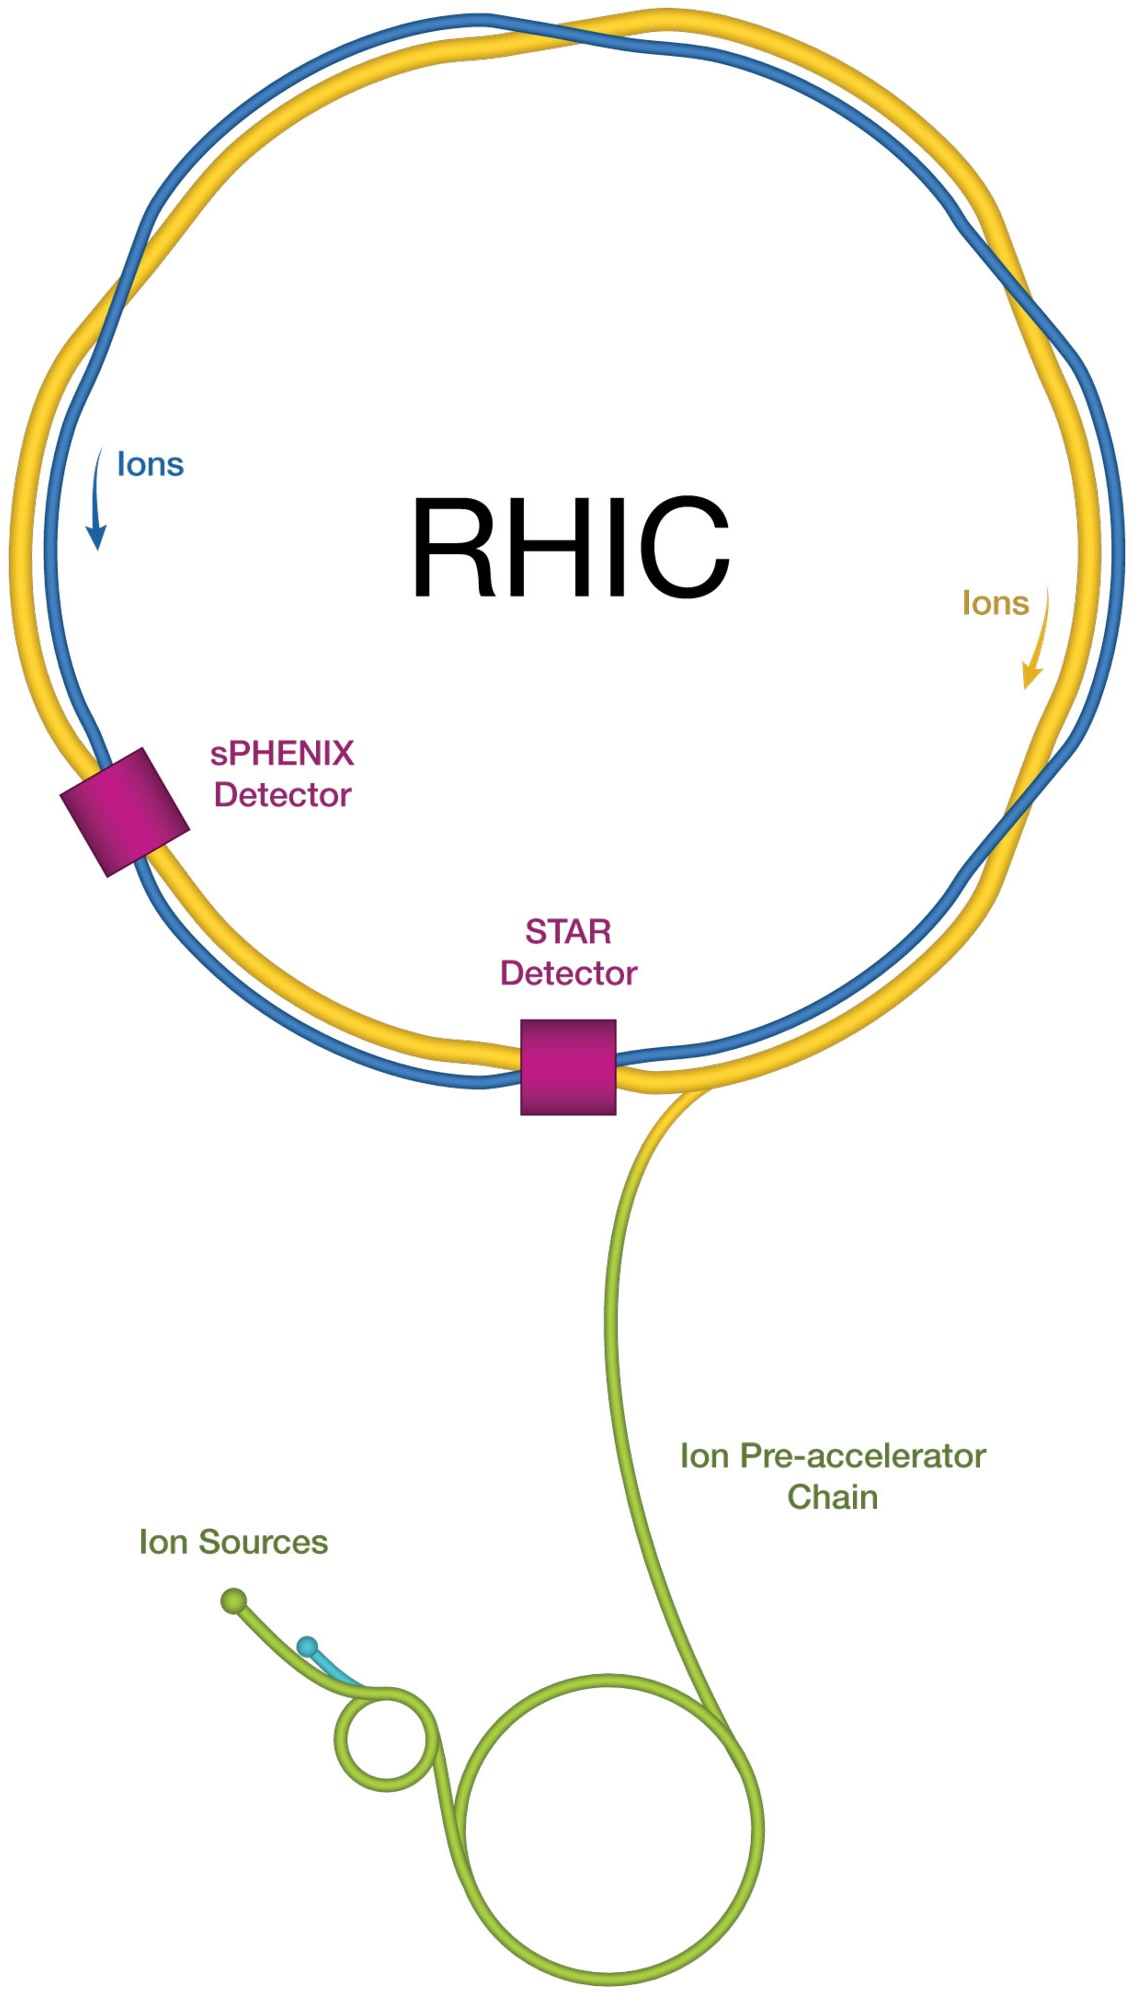
\includegraphics[height=10.4cm]{img/rhic.jpg}
        \caption{[cite RHIC image]}
        \label{fig:eic:comparison::rhic}
    \end{subfigure}
    %\hspace{0.02\linewidth}
    \raisebox{20\height}{\Huge$\rightarrow$}
    %\hspace{0.02\linewidth}
    \begin{subfigure}{0.52\linewidth}
        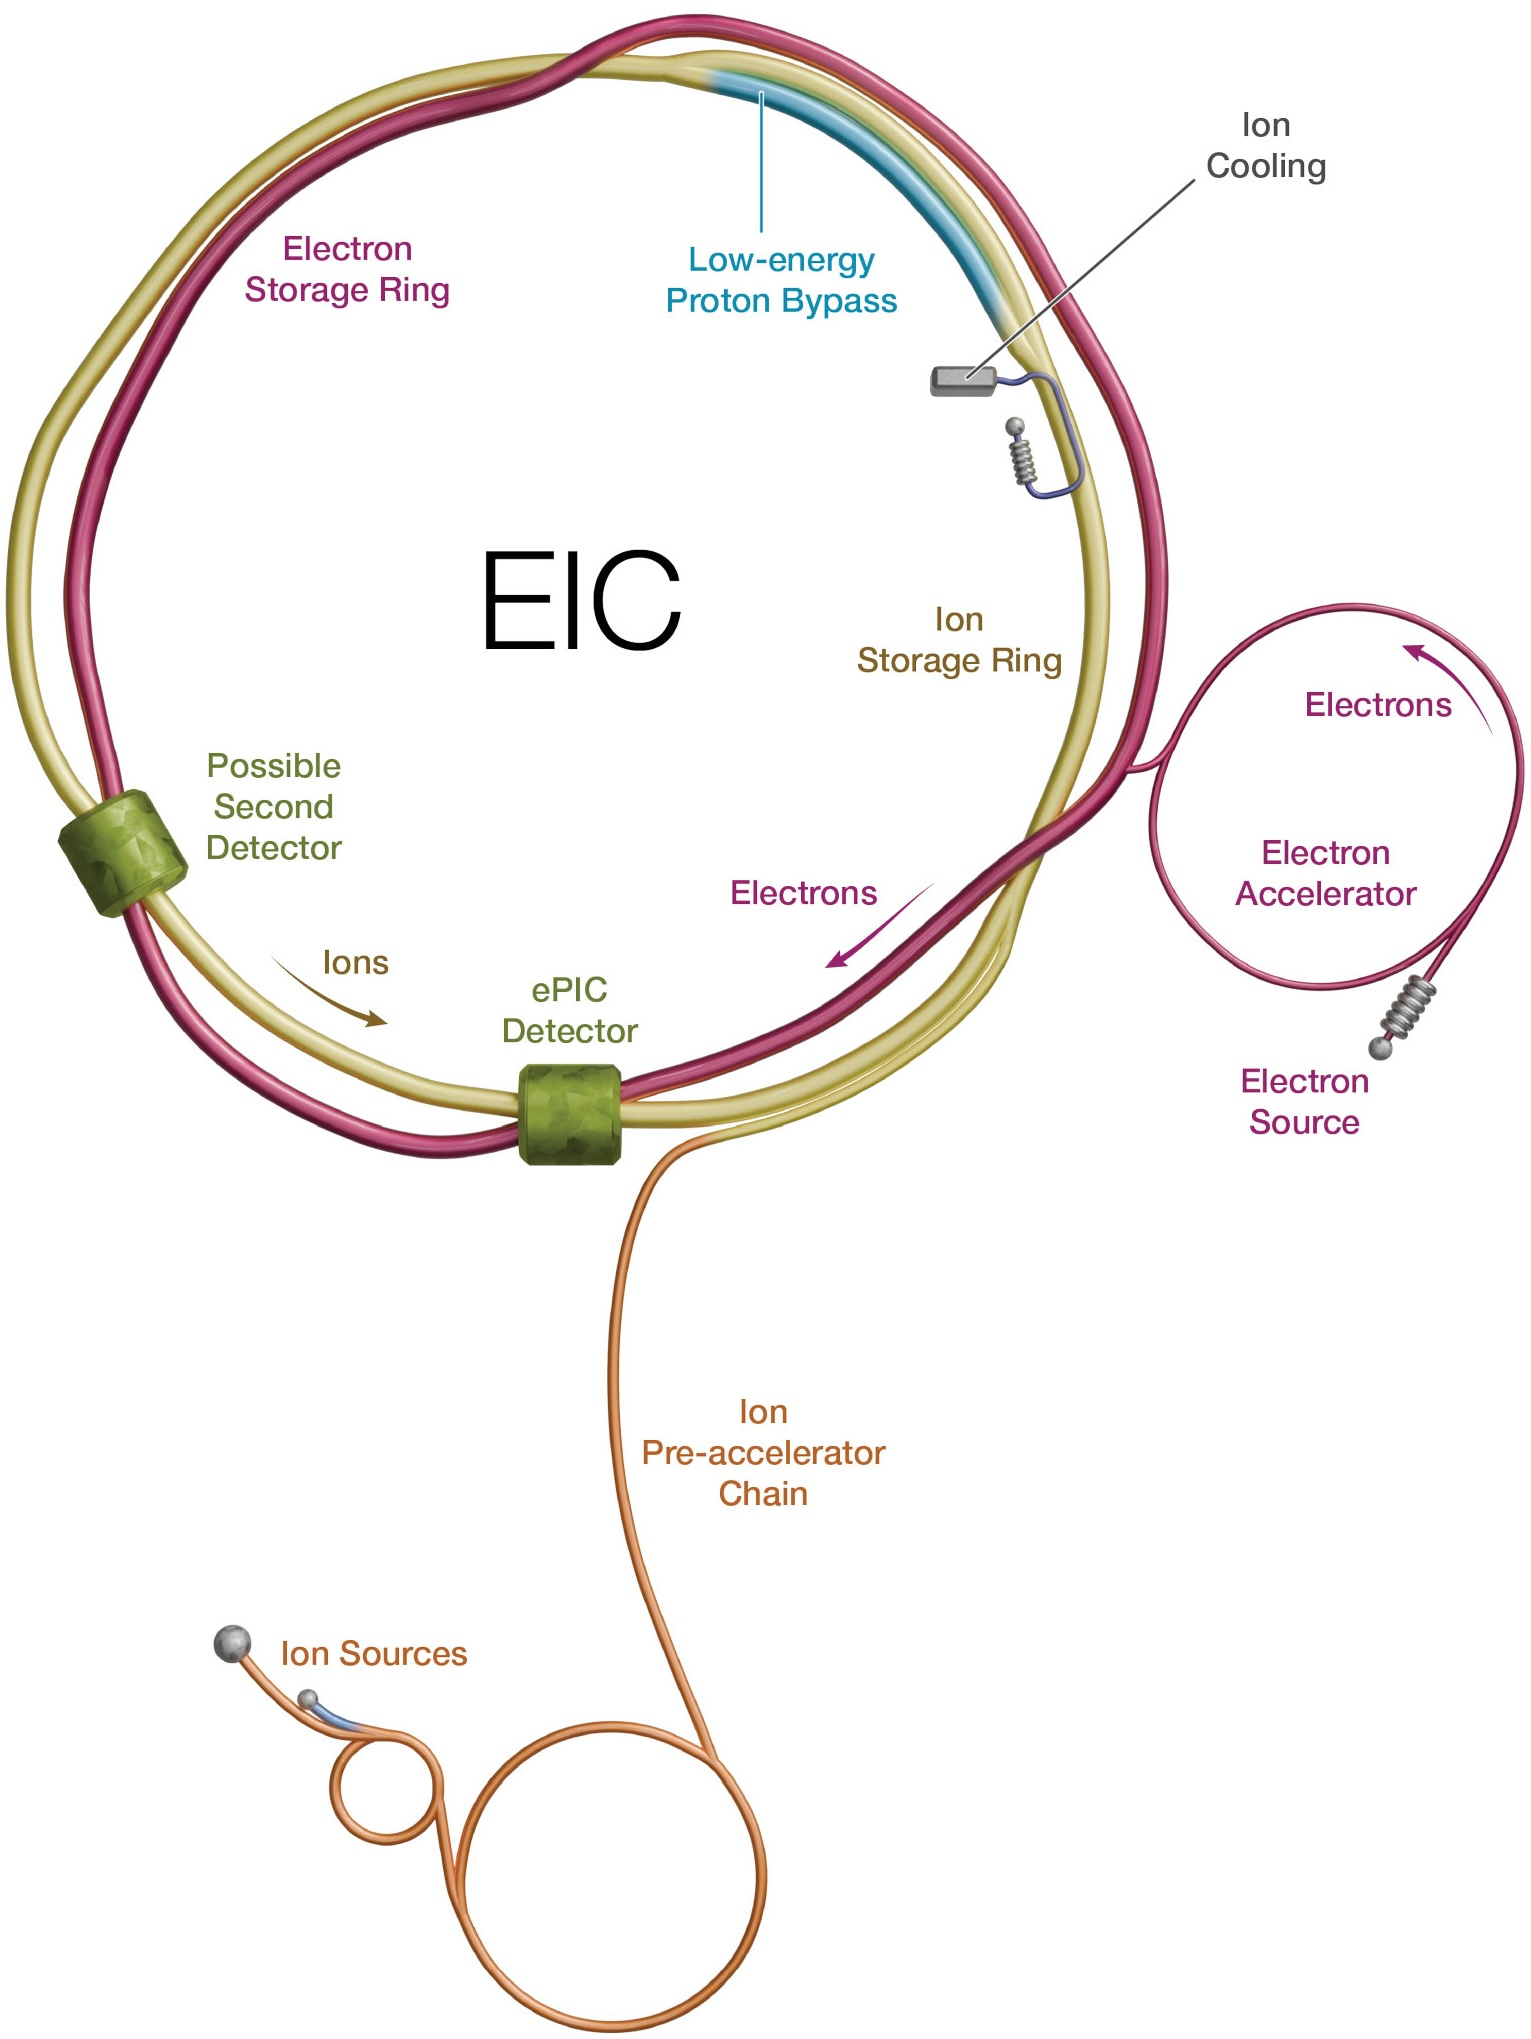
\includegraphics[height=10.4cm]{img/eic.jpg}
        \caption{[cite EIC image]}
        \label{fig:eic:comparison::eic}
    \end{subfigure}
    \caption{(a) Layout of the existing RHIC facility. (b) Conceptual design of EIC.}
    \label{fig:eic:comparison}
\end{figure}


% \section{Current Design Plan}

% \textit{the changes from usual illustrations (copied)}:\\
% In 2024, the project made several key EIC design decisions. They will lead to
% formal Project Scope changes after the Technical Change Control Board (TCCB)
% and the CCB processes.
% \begin{enumerate}[topsep=1mm, itemsep=0mm]
%     \item Reuse the entire Yellow RHIC ring, delay the 41-GeV bypass (a Blue RHIC arc).
%     \item Implement a new room-temperature Hadron Storage Ring (HSR) injection line.
%     \item Drop Strong Hadron Cooling (SHC), add Low-Energy Cooling (LEC).
%     \item Move the Rapid Cycling Synchrotron (RCS) out of the collider tunnel.
%     \item Delay the 28 nC/bunch and the 18 GeV capability implementation (ESR and RCS).
% \end{enumerate}
% These design decisions resolve uncertainties, challenges, and risks to EIC
% performance, safety, and future operation and maintenance. [Nagaitsev Frascati]



% maybe will fit better in another chapter

% \section{Advantages? \textit{Prínosy}}

% \section{Second detector?}
% is anyone seriously working on it, or is it too soon to care?

% \begin{figure}[H]
%     \centering
%     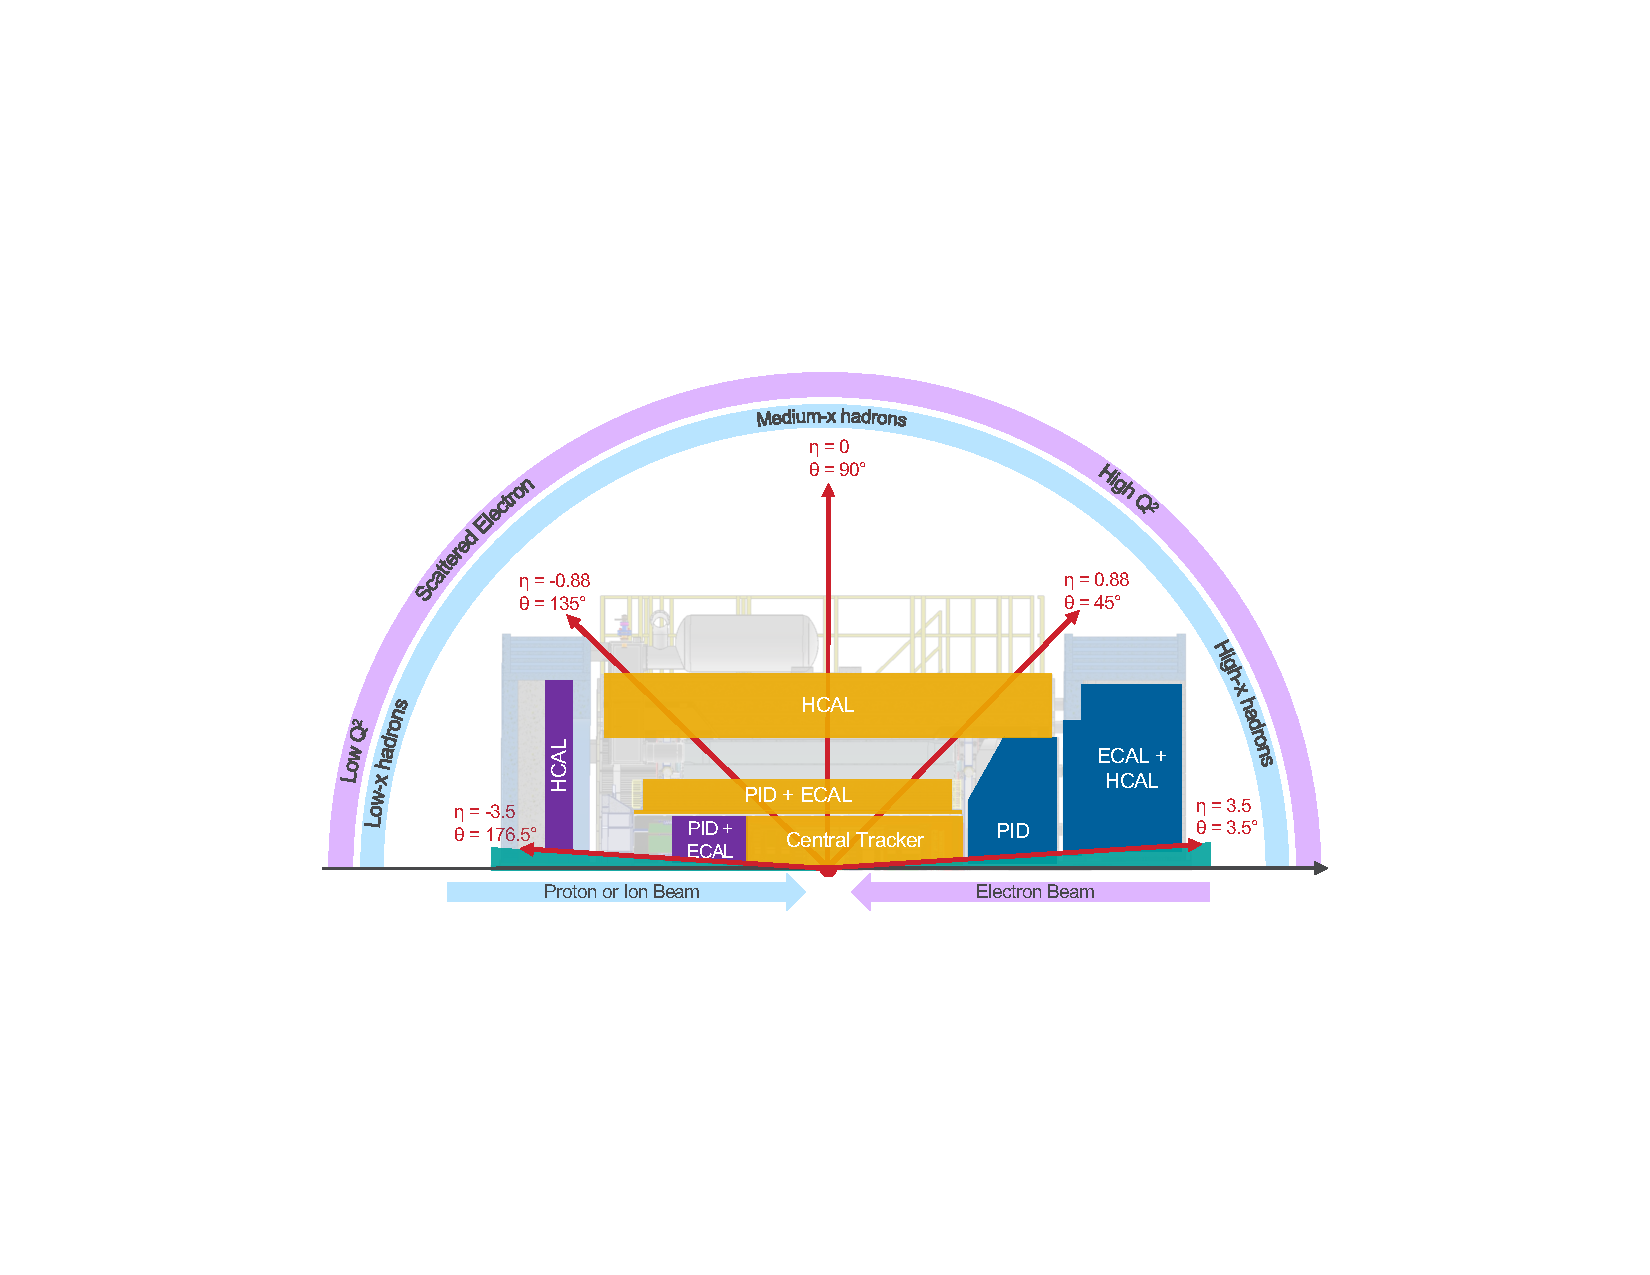
\includegraphics[width=.8\linewidth]{img/range.pdf}
%     \caption{always this image \url{https://doi.org/10.5281/zenodo.14939545}}
%     \label{fig:eic:range}
% \end{figure}
% \newpage

%%%%%%%%%%%%%%%%%%%%%%%%%%%%%%%%%%%%%%%%% kapitola Physics %%%%%%%%%%%%%%%%%%%%%%%%%%%%%%%%%%%%%%%%%%%%%%%%%%%%%%%

% \newpage 
%\chapter{Physics}\label{cha:physics} % chktex 24

\section{Deep Inelastic Scattering?}
PDFs, GPDs

scaling (pointlikeness), scaling violation

$\cev{v}^{2}$
$\cev{v}^2$
$\vec{v}\na{'}$
Callan-Gross (spin 1/2)

Bjorken scaling violation - dependence on Q2 at low x

\begin{figure}[H]
    \centering
    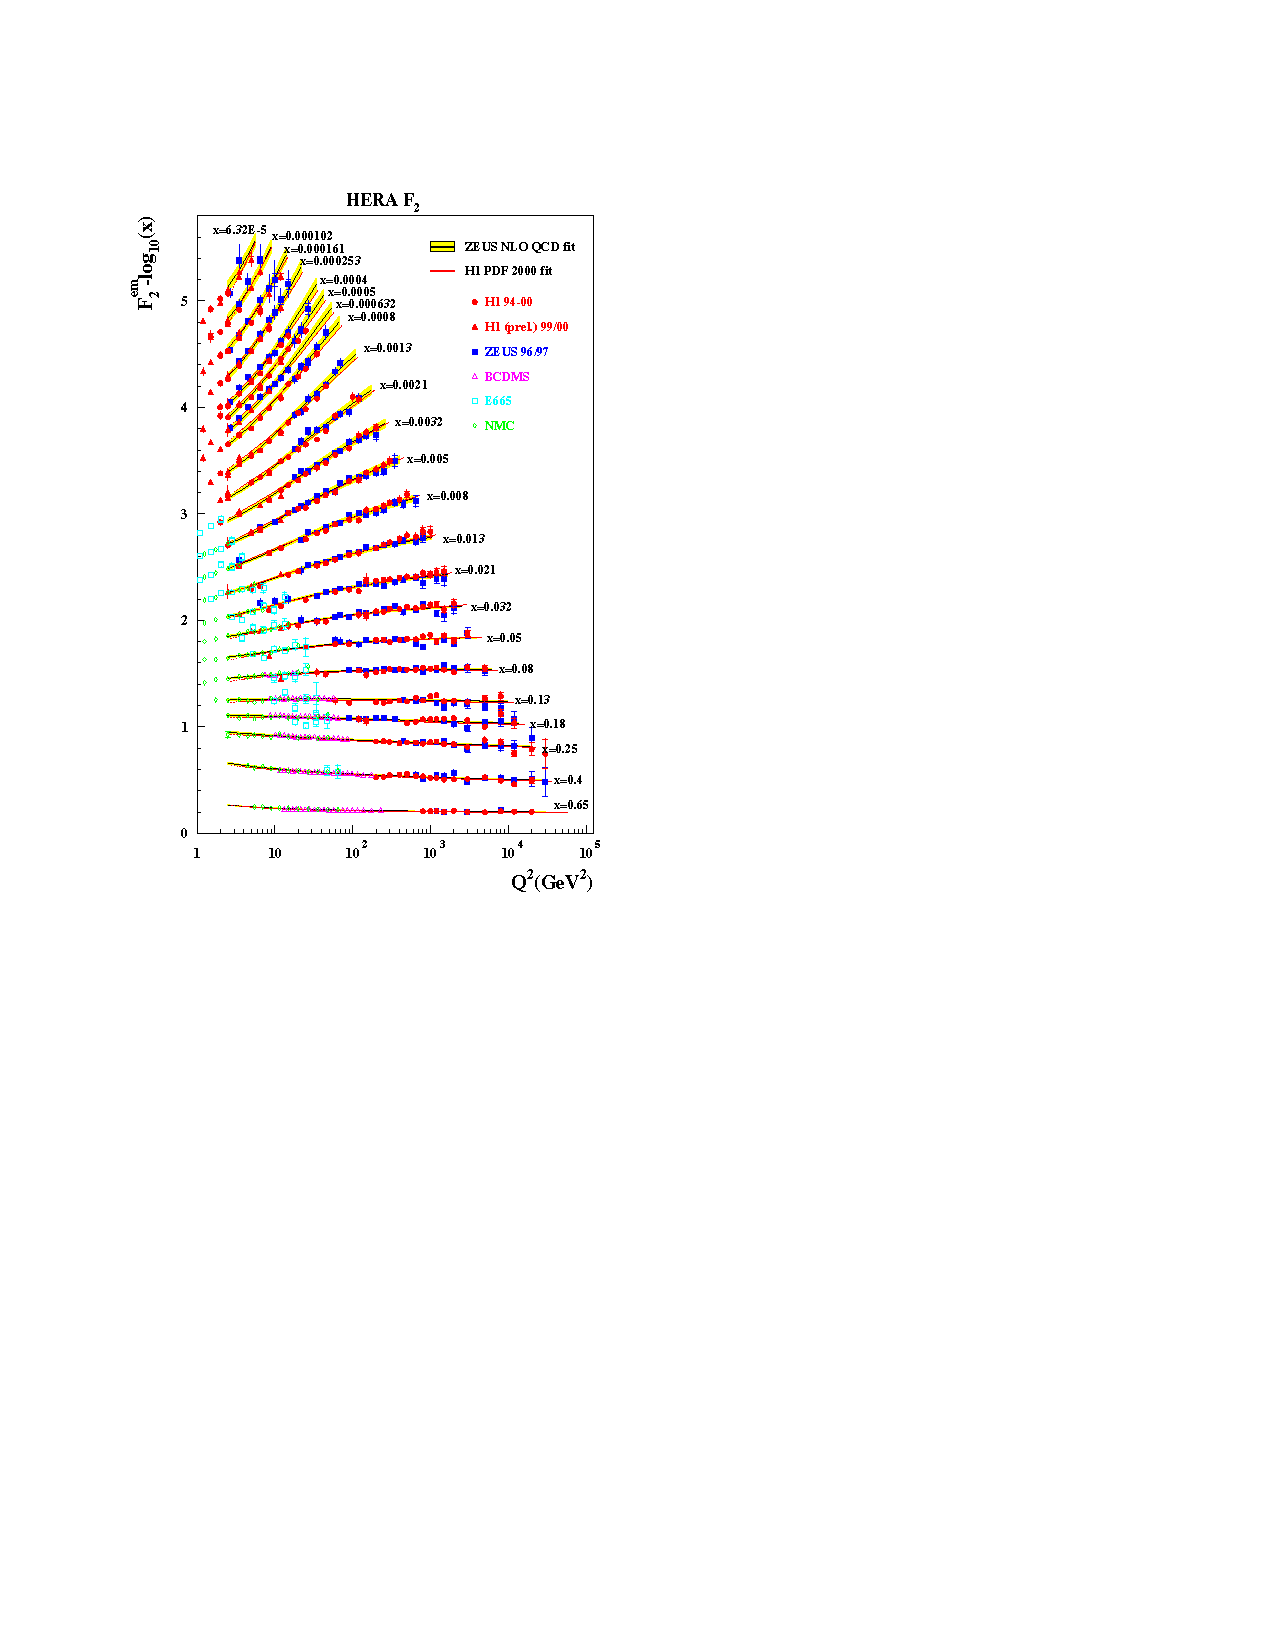
\includegraphics[width=.7\linewidth]{img/scaling_violation.pdf}
    \caption{[cite scaling violation]}
    \label{fig:physics:scaling_violation}
\end{figure}

\section{Diffractive vector-meson production}
Generalized Parton Distributions in ePIC, 


% \newpage

%%%%%%%%%%%%%%%%%%%%%%%%%%%%%%%%%%%%%%%% kapitola ePIC %%%%%%%%%%%%%%%%%%%%%%%%%%%%%%%%%%%%%%%%%%%%%%%%%%%%%%%


% \newpage 
%\chapter{ePIC Experiment}\label{cha:ePIC} % chktex 24
% \newpage

%%%%%%%%%%%%%%%%%%%%%%%%%%%%%%%%%%%%%%%% kapitola nHCal %%%%%%%%%%%%%%%%%%%%%%%%%%%%%%%%%%%%%%%%%%%%%%%%%%%%%%%%%%%%


% \newpage 
%\chapter{nHCal}\label{cha:nHCal} % chktex 24
extensively from pre-TDR - new iteration in two weeks - is it worth the wait?

WHERE IS THE GOOGLE DOC? 

Overview from some Leszek's presentation? is Leszek relevant?

\section{Motivation}
still tail catcher of nECal (what is that really, only of that?)

start with HERA (maybe) - then continue from that ("to not make the same mistake")

Vector meson - the matrix image + the 012K plots

only for e + Au and phi, or also e + p, and J/psi?

\section{Construction}
realistic dimensions and location

tiling? is it really important?

does clustering make sense to mention? - probably somewhere else (simulations)

changes?

sampling, N layers, ... ok, but what about material e.g.?

sampling fraction - possible to be compensating (Elke says NO)? what did Subhadip prove, then? - how achieved? how calculated?

but what about true construction? does Leszek now? does anybody?

two images from BP? or something else? cite myself?

anything about neutrons? meaningful?

is tilt usable? if for VU, also for DP?

\section{?}





% \newpage

%%%%%%%%%%%%%%%%%%%%%%%%%%%%%%%%%%%%%%%% kapitola Tools %%%%%%%%%%%%%%%%%%%%%%%%%%%%%%%%%%%%%%%%%%%%%%%%%%%%%%%%%%%%


% \newpage 
% \
% \newpage

%%%%%%%%%%%%%%%%%%%%%%%%%%%%%%%%%%%%%%%% kapitola WORK %%%%%%%%%%%%%%%%%%%%%%%%%%%%%%%%%%%%%%%%%%%%%%%%%%%%%%%%%


% \newpage 
%\chapter{Practical work}\label{cha:work} % chktex 24


\section{Material plots?}
\begin{figure}[H]
    \centering
    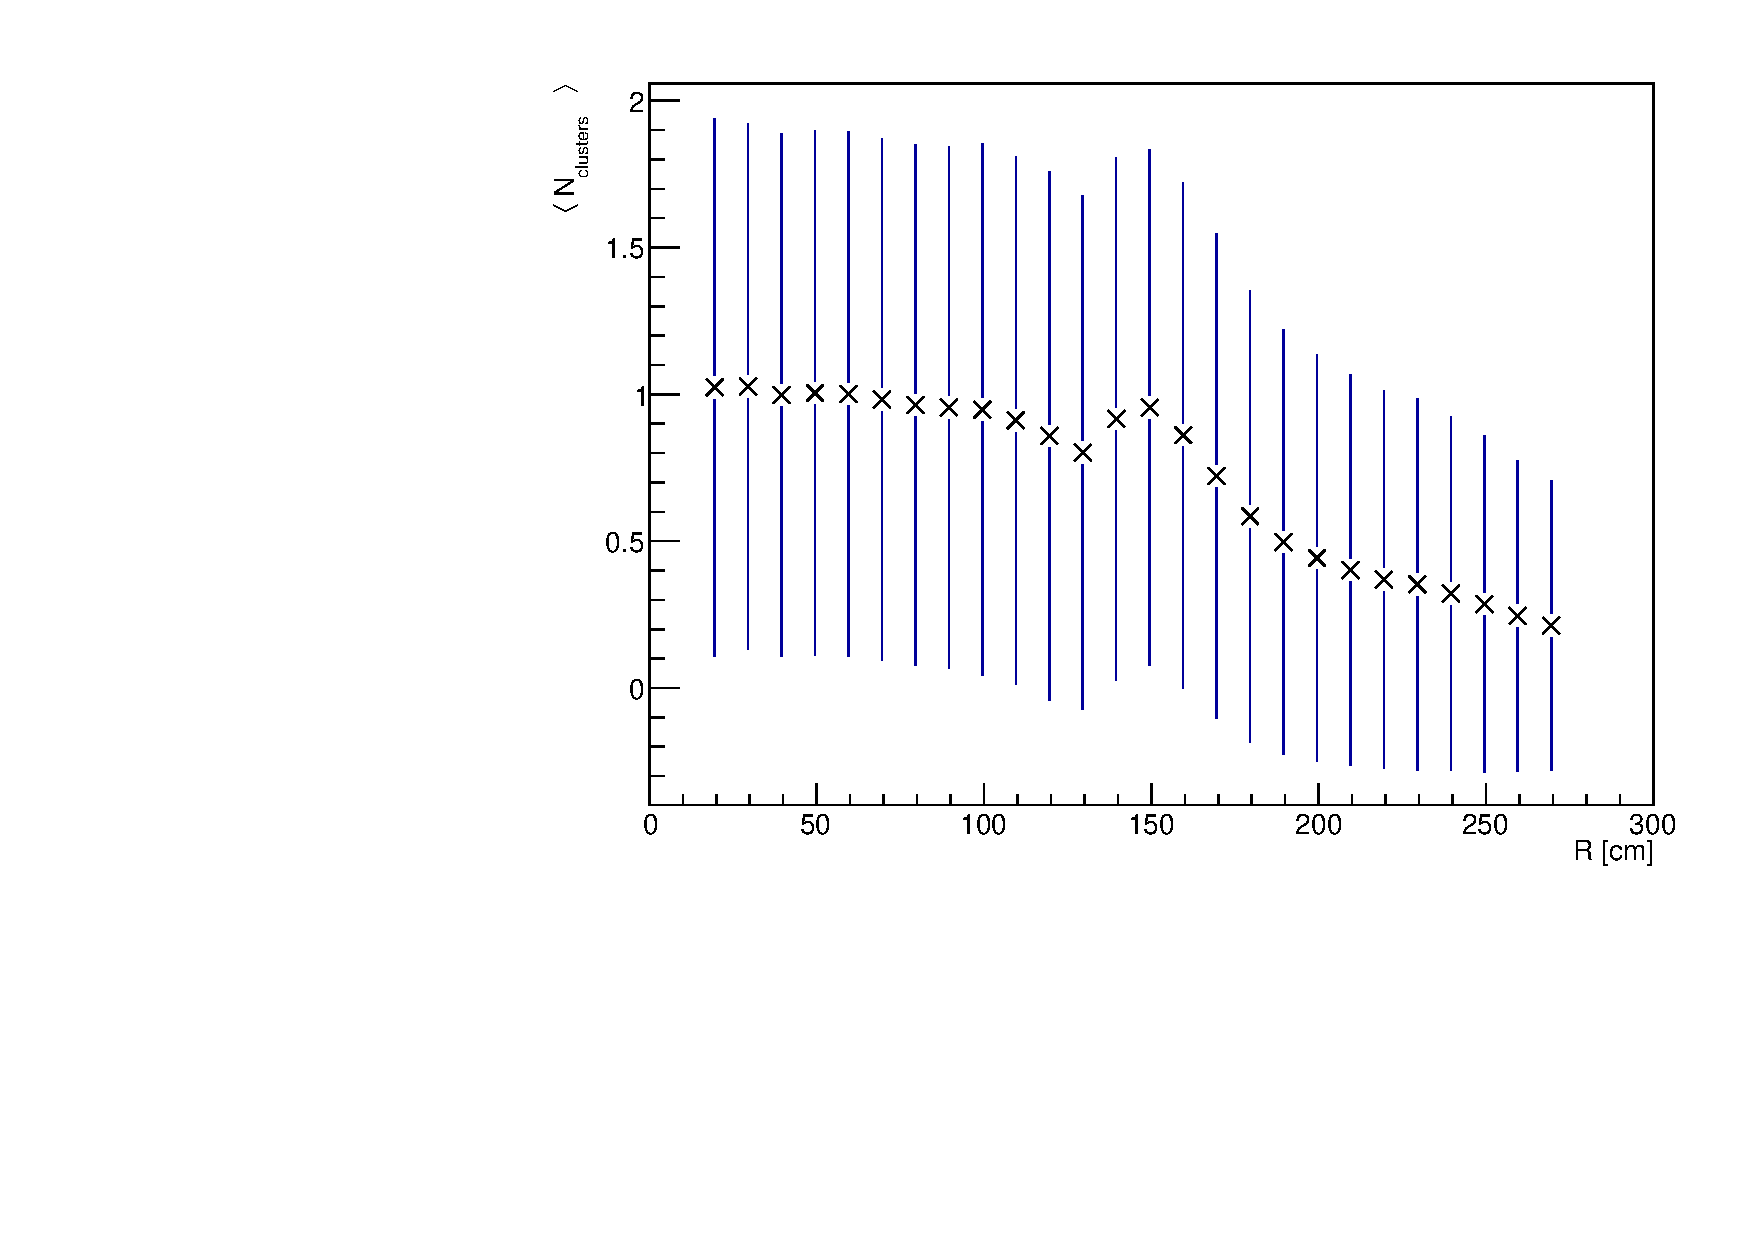
\includegraphics[width=.6\linewidth]{img/averageClusters.pdf}
    \caption{average clusters}
    \label{fig:work:average}
\end{figure}
labels too small
\begin{figure}[H]
    \centering
    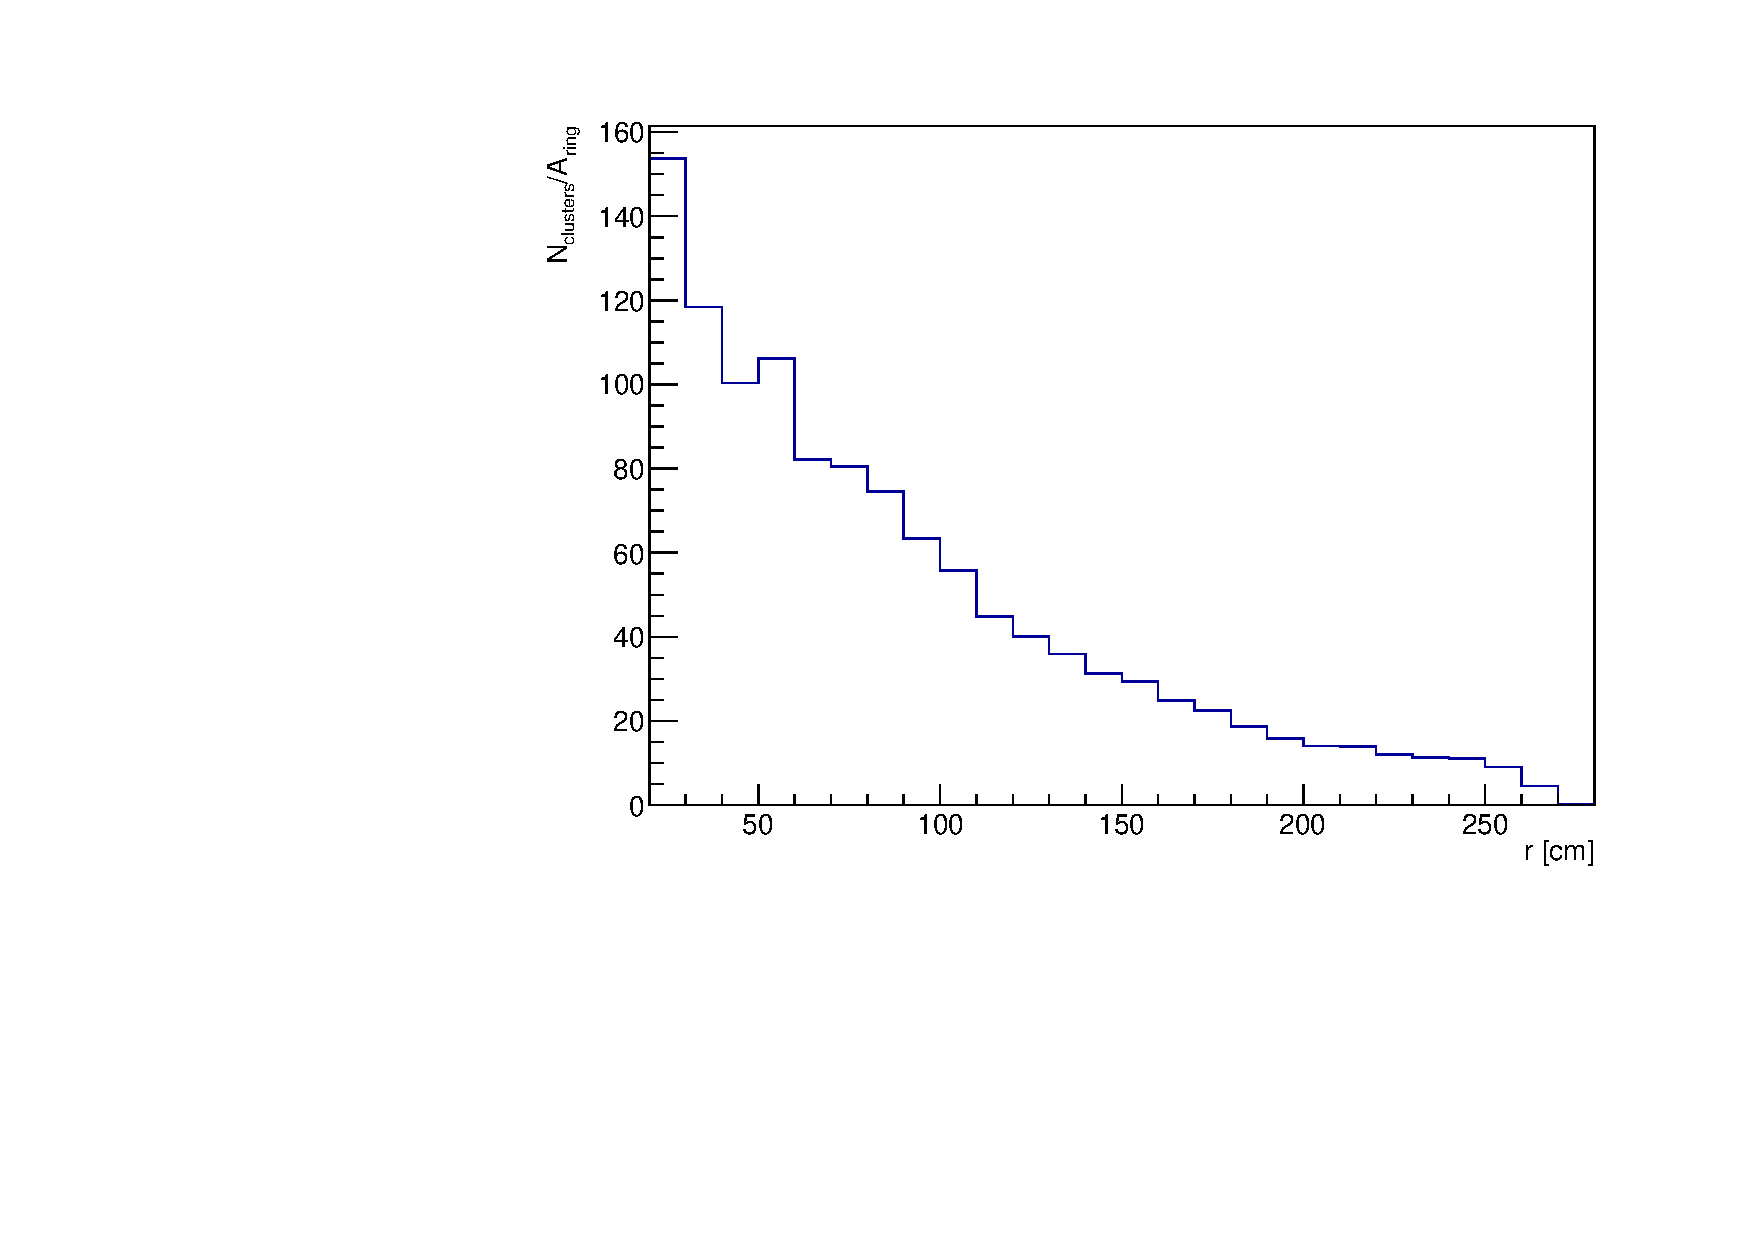
\includegraphics[width=.6\linewidth]{img/combined_clusters_norot.pdf}
    \caption{combined clusters}
    \label{fig:work:combined}
\end{figure}


\section{tilt?}
\begin{figure}[H]
    \begin{subfigure}{.48\linewidth}
        \centering
        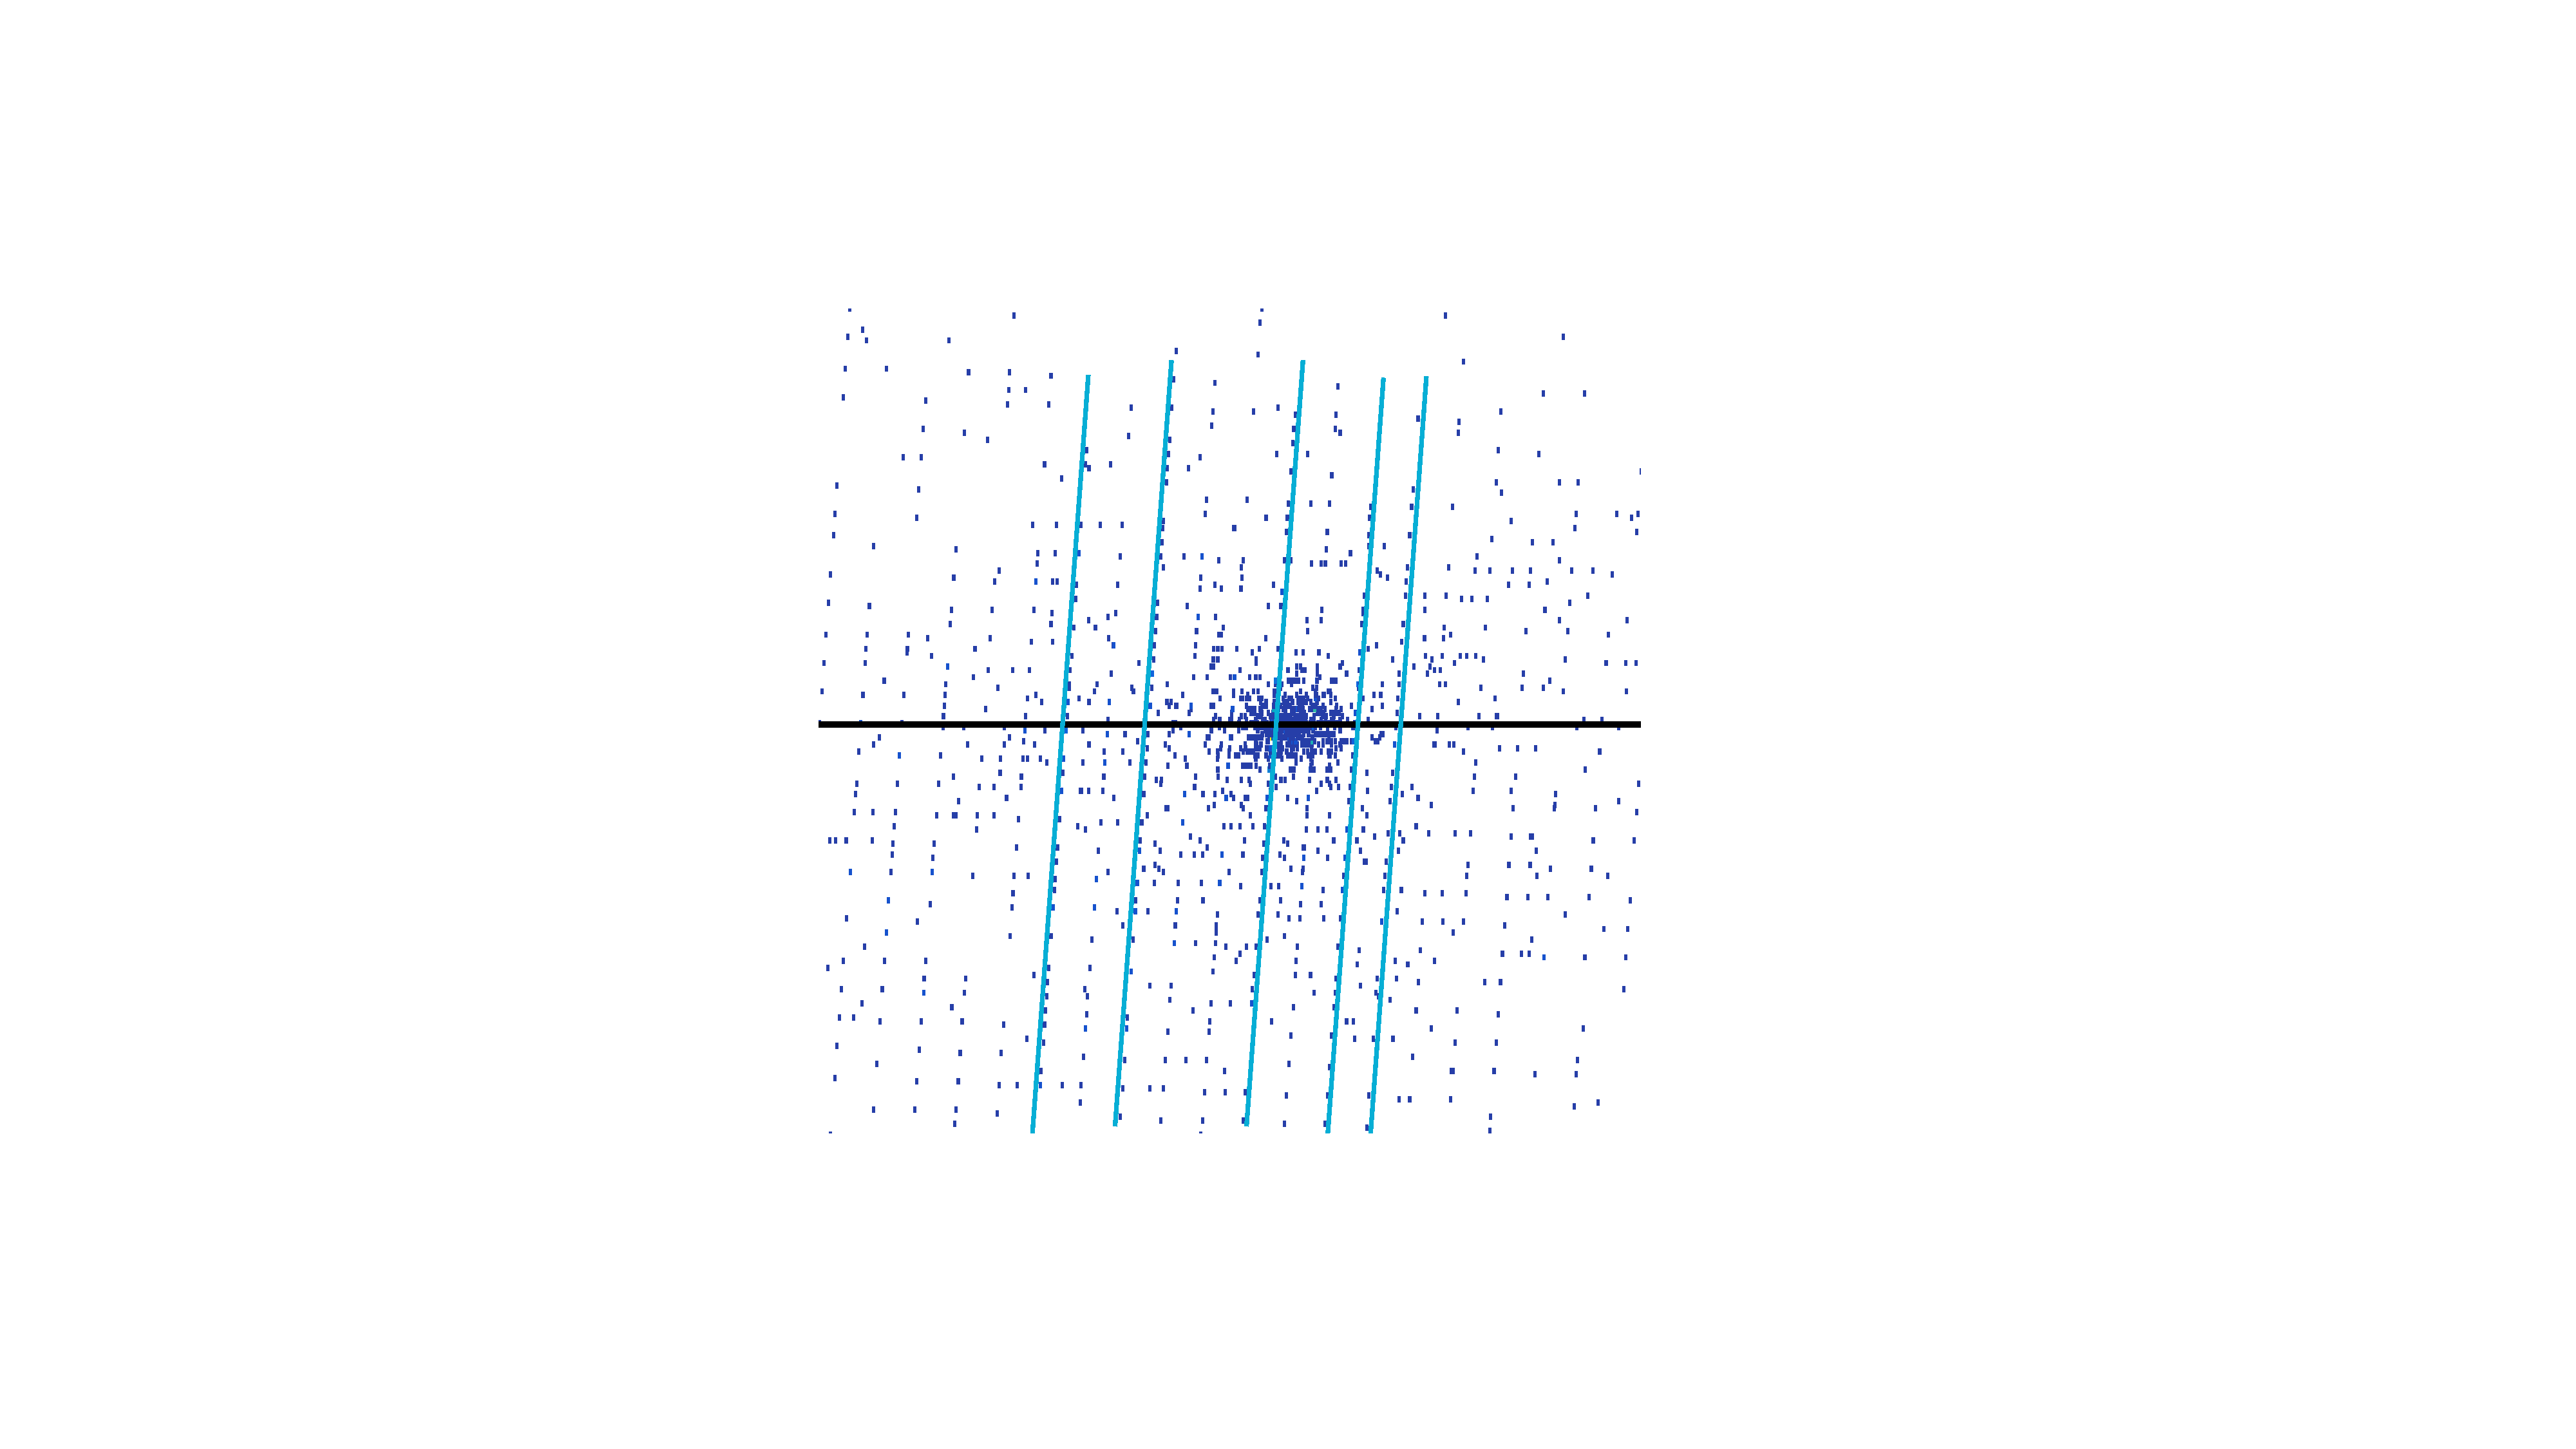
\includegraphics[width=\linewidth]{img/orig_config_clusters.pdf}
        \caption{before}
        \label{fig:work:tilt:before}
    \end{subfigure}
    \begin{subfigure}{.48\linewidth}
        \centering
        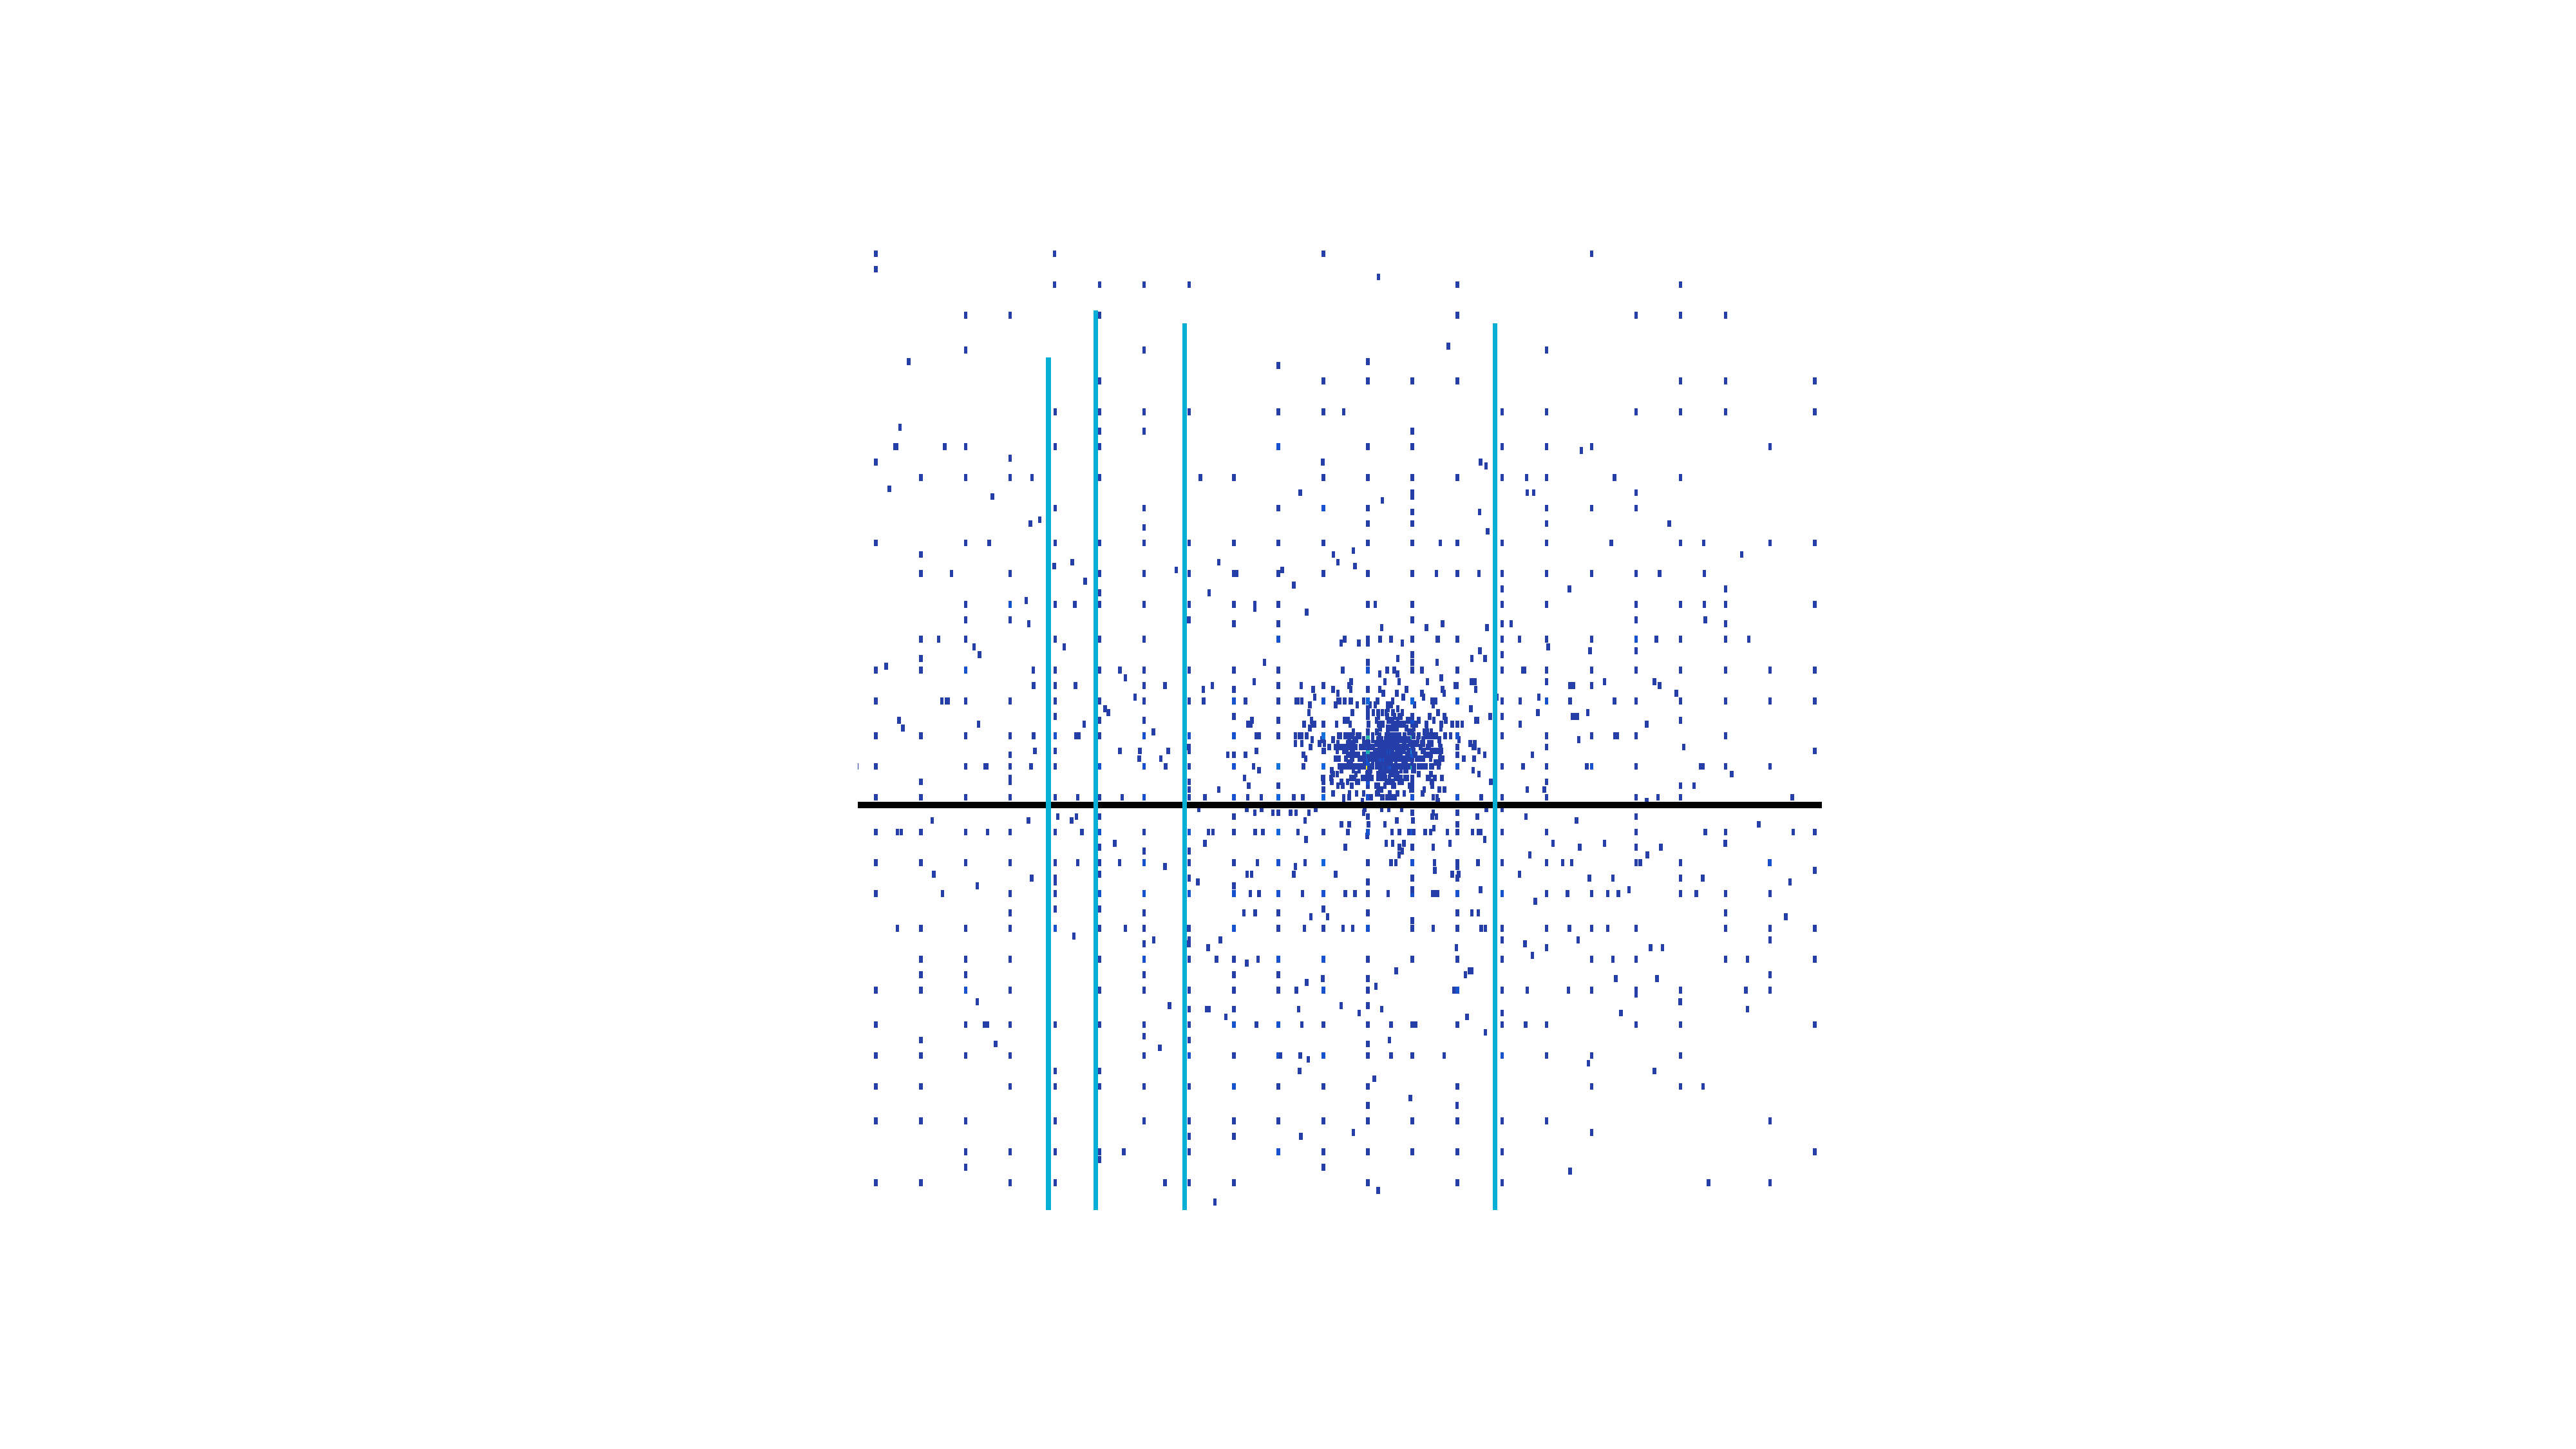
\includegraphics[width=\linewidth]{img/every_rot_removed_clusters.pdf}
        \caption{after}
        \label{fig:work:tilt:after}  
    \end{subfigure}
    \caption{need to level the lines, if decided to keep}
    \label{fig:work:tilt}
\end{figure}

\section{Sar$t$re MC generator}

\url{https://github.com/eic/SARTREdataset/blob/main/runcards/sartre_bnonsat_Au_phi.txt}

info about Campaign simulations

\section{phi - KK plots}
% \newpage

%%%%%%%%%%%%%%%%%%%%%%%%%%%%%%%%%%%%%%%%%%%%%% Zaver %%%%%%%%%%%%%%%%%%%%%%%%%%%%%%%%%%%%%%%%%%%%%%%%%%%%%%%%%%%%%%

% \newpage
\chapter*{Summary}\label{cha:outro} % chktex 24
\addcontentsline{toc}{chapter}{Summary}

if it's meant to be then it will be\\

\textbf{NEED TO INCORPORATE REFs FROM ASSIGNMENT:}\\

[1] R. Abdul Khalek et al., Snowmass 2021 White Paper: Electron Ion Collider for High Energy Physics, arXiv:2203.13199\\
\textbf{!} \textit{the required physics is probably still more or less relevant}\\

[2] EIC User Group,  White Paper on the Electron-Ion Collider in Preparation for the NSAC Long Range Plan, Zenodo (2023), \url{https://doi.org/10.5281/zenodo.7500024}\\
\textbf{!} \textit{what is the difference between this and [1]?}\\

[3] D. Boer et al., Physics case for quarkonium studies at the Electron Ion Collider, arXiv:2409.03691\\
\textbf{!} \textit{maybe useful for something about the $\phi$s? doesn't have the good feynman diagram}\\

[4] Ch. Montag, Status of the Electron-Ion Collider, PoS SPIN2023 (2024) 135\\
\textbf{!} \textit{ten pages long, 25th International Spin Physics Symposium (SPIN 2023) 24-29 September 2023 (proceedings) - old and probably severely outdated $\rightarrow$ useful MAYBE only for the most basic facts (luminostity, used particle species...)}\\

[5] P. Antonioli, The European Participation to the Electron Ion Collider, Nucl.Phys.News 34 (2024) 3, 21-25\\
\textbf{!} \textit{not sure what can be used from this - czech manufacture of crystals?}


% \newpage



%%%%%%%%% Literatura %%%%%%%%%%%%
\urlstyle{same}
% \thispagestyle{plain}
\begin{thebibliography}{60}
\addcontentsline{toc}{chapter}{Bibliography}

    \bibitem{YR} R. Abdul Khalek et al., "Science Requirements and Detector Concepts for the Electron-Ion Collider: EIC Yellow Report," \textit{Nuclear Physics A}, vol. 1026, a. 122447, October 2021. [Online]. Available: \url{https://doi.org/10.1016/j.nuclphysa.2022.122447}. [Accessed: 20-Dec-2023].

    \bibitem{wiki} ePIC Collaboration, "ePIC Experiment Wiki," \textit{wiki.bnl.gov}, 2024. [Online]. Available: \url{https://wiki.bnl.gov/EPIC/index.php?title=Main_Page}. [Accessed: 27-Feb-2024].

    \bibitem{rhic} Brookhaven National Laboratory, "Relativistic Heavy Ion Collider webpage," \textit{www.bnl.gov}, 2024. [Online]. Available: \url{https://www.bnl.gov/rhic}. [Accessed: 23-Jul-2024].

    \bibitem{whitepaper} A. Accardi et al., "Electron-Ion Collider: The next QCD frontier," \textit{The European Physical Journal A}, vol. 52, a. 268, 2016. [Online]. Available: Springer Link, \url{http://www.springer.com} [Accessed: 20-Dec-2023].

    \bibitem{CDR} U.S. Department of Energy, "Electron Ion Collider Conceptual Design Report 2021," \textit{technical report}, 2021. [Online] Available: \url{https://doi.org/10.x2172/1765663}. [Accessed: 05-Apr-2024].

    \bibitem{grupen_wigmans} R. Wigmans, "Calorimetry," in \textit{Handbook of Particle Detection and Imaging}, C. Grupen and I. Buvat, Eds. Berlin, Heidelberg: Springer, 2012, pp. 497-517. [Online]. Available: \url{https://doi.org/10.1007/978-3-642-13271-1_20}. [Accessed: 12-Apr-2024].

    \bibitem{livan_calorimetry} M. Livan and R. Wigmans, \textit{Calorimetry for Collider Physics, an Introduction}. Cham: Springer, 2019. 

    \bibitem{grupen_particle-detectors} C. Grupen and B. A. Shwartz, \textit{Particle Detectors}. 2nd ed. Cambridge: Cambridge University Press, 2008.

    \bibitem{hanagaki} K. Hanagaki, J. Tanaka, M. Tomoto and Y. Yamazaki, "Particle Identification," in \textit{Experimental Techniques in Modern High-Energy Physics: A Beginner‘s Guide}, K. Hanagaki, J. Tanaka, M. Tomoto and Y. Yamazaki, Eds. Tokyo: Springer. 2022, pp. 69-114. [Online]. Available: \url{ https://doi.org/10.1007/978-4-431-56931-2_6}. [Accessed: 12-Apr-2024].

    \bibitem{lippmann} Ch. Lippmann, "Particle Identification," \textit{Nuclear Instruments and Methods in Physics Research Section A: Accelerators, Spectrometers, Detectors and Associated Equipment}, vol. 666, pp. 148-172, February 2012. [Online]. Available: \url{https://doi.org/10.1016/j.nima.2011.03.009}. [Accessed: 12-Apr-2024].

    \bibitem{dd4hep} M. Frank, F. Gaede, M. Petric and A. Sailer, "DD4hep webpage" \textit{dd4hep.web.cern.ch}, 2023. [Online] Available: \url{https://dd4hep.web.cern.ch/}. [Accessed: 02-May-2024].

    \bibitem{DD4hepManual} M. Frank, F. Gaede, M. Petric and A. Sailer, "DD4hep User Manual," July 24, 2024. [Online] Available: \url{https://dd4hep.web.cern.ch/dd4hep/usermanuals/DD4hepManual/DD4hepManual.pdf}. [Accessed: 02-Jun-2024].

    \bibitem{JANA2} D. Lawrence, A. Boehnlein, N. Brei and D. Romanov, "JANA2: Multithreaded Event Reconstruction," \textit{Journal of Physics: Conference Series}, vol. 1525, a. 012032, 2020. [Online] Available: \url{https://dx.doi.org/10.1088/1742-6596/1525/1/012032}. [Accessed: 02-Jul-2024].

    \bibitem{eicrecon_page} "EICrecon webpage," [Online]. Available: \url{https://eic.github.io/}. [Accessed: 23-May-2024].

    \bibitem{hepmc3} A. Buckley et al., "The HepMC3 event record library for Monte Carlo event generators," \textit{Computer Physics Communications}, vol. 260, a. 107310, March 2021. [Online]. Available: \url{https://doi.org/10.1016/j.cpc.2020.107310}. [Accessed: 02-Jul-2024].

    \bibitem{podio} AIDAsoft, "podio GitHub repository," \textit{github.com}, 2024. [Online]. Available: \url{https://github.com/AIDASoft/podio}. [Accessed: 22-Jul-2024].
     
\end{thebibliography}

% \bibliography{bib_ref.bib}
% \bibliographystyle{unsrt} % nebo něco jinýho, podle toho stylu co je potřeba (stačí googlit)


%%%%%%%%%%  Prilohy  %%%%%%%%%%%%%%%%%%   

%\input{kapitoly/appendix}


\end{document}
